\chapter{Технологический раздел}
\section{Выбор среды разработки}

\subsection{Общие сведения}
\label{sec:soft_description:general}

Для функционирования программы необходимо следующее программное обеспечение:
\begin{itemize}
\item Python 2.5.2;
\item Django 1.1.1;
\item Apache 2.2.14 с модулем mod\_python, WebDAV;
\item Поддерживаемая Django СУБД: PostgreSQL версии 8.2 или выше, MySQL 4.1/5.0, Oracle версии 9i или выше, SQLite версии 3.3.6 или выше; возможно использование других СУБД при наличии соответствующего интерфейса (см.~\url{http://docs.djangoproject.com/en/dev/ref/databases/#using-a-3rd-party-database-backend}, 2009);
\item Одна или несколько систем контроля версий: Subversion 1.6.3, Git 1.6.5;
\item Одна или несколько систем управления проектами (на данный момент поддерживается Trac 0.11.5).
\end{itemize}

Программа написана полностью на языке \Soft{Python} (\url{http://www.python.org}, 2009) с использованием веб-фреймворка \Soft{Django} (\url{http://www.djangoproject.com}, 2009). Все вышеперечисленное ПО (за исключением СУБД Oracle) является свободным и кроссплатформенным.

\subsection{Функциональное назначение}

\subsection{Описание логической структуры}

В данном разделе дано описание основных модулей программного комплекса, а также содержащихся в них классов, функций и переменных.

%\input{api_rus/iu7dev.frontends-module}



\subsection{Используемые технические средства}
\label{sec:soft_description:tech}

В состав технических средств должна входить ЭВМ, включающая в себя:
\begin{itemize}
    \item процессор архитектуры, поддерживаемой UNIX-подобными ОС: \Code{amd64}, \Code{i386}, \Code{ia64}, \Code{MIPS}, \Code{ARM}, \Code{ppc}, \Code{sparc64}, \Code{sun4v}, \Code{xbox};
    \item оперативную память объемом не менее 64МБ;
    \item не менее 30МБ свободного места на диске для установки комплекса, а также дополнительное место для базы данных (не менее 50МБ).
\end{itemize}

\subsection{Вызов и загрузка}

Для установки комплекса на сервер необходимо выполнить следующие команды из каталога проекта:

\begin{lscommand}\verb+./conf/global_init.sh+\end{lscommand}

\noindentДанный скрипт совершает все необходимые действия по созданию работающего веб-приложения, конфигурации базы данных и веб-сервера. После его выполнения система сразу начинает работу. Во время выполнения скрипта при необходимости могут быть запрошены данные, например, пути к каталогам, в которых будут размещены архивы проектов, а также имя виртуального хоста, которое используется при конфигурации Apache. После успешного завершения установки, административный интерфейс доступен по относительному URL-адресу \Code{/admin/}, главная страница пользовательского интерфейса -- по адресу \Code{/}.

\section{Руководство пользователя}
\label{sec:man}

\subsection{Назначение программы}


\subsection{Условия выполнения программы}

Минимальный состав технических средств описан в разделе \ref{sec:soft_description:tech}.

Минимальный состав программных средств описан в разделе \ref{sec:soft_description:general}.

\subsection{Выполнение программы}

\label{sec:workorder}

На рисунке~\ref{fig:main_page} представлена главная страница системы голосовой аутентификации. Справа расположен логотип системы, под которым отражается статус пользователя (авторизован или нет). В центральной части страницы находится ссылка для перехода на страницу аутентификации и форма ввода имени учетной записи.
В нижней части представлена "Навигация", которая состоит из ссылки на регистрацию в системе и ссылки для перехода на главную страницу защищаемого интернет-ресурса. Если пользователь не авторизован на интернет-ресурсе, то в списке "Навигация" присутствует ссылка на страницу с формой ввода имени учетной записи и пароля. Если пользователь авторизован, то вместо ссылки на страницу с формой ввода имени учетной записи и пароля присутствует ссылка "Выход".

\begin{figure}[hbt!]
\center{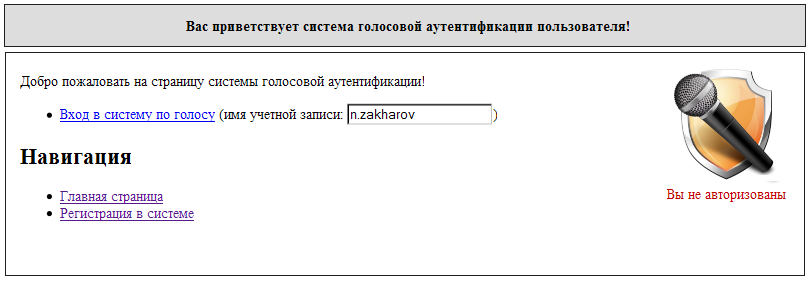
\includegraphics{static_include/main_page.png}}
\caption{Главная страница системы голосовой аутентификации}
\label{fig:main_page}
\end{figure}

При выборе пункта "Регистрация в системе" пользователь автоматически переходит на страницу, которая содержит список требований, удовлетворение которых необходимо для регистрации в системе. Если пользователь авторизован на интернет-ресурсе, на странице присутствует ссылка для перехода к созданию персональной голосовой модели (рисунок~\ref{fig:enrollment_initial_authentificated}). Если пользователь не авторизован, на странице отображается сообщение о необходимости авторизации (рисунок~\ref{fig:enrollment_initial_anonymous}).

\begin{figure}[hbt!]
\center{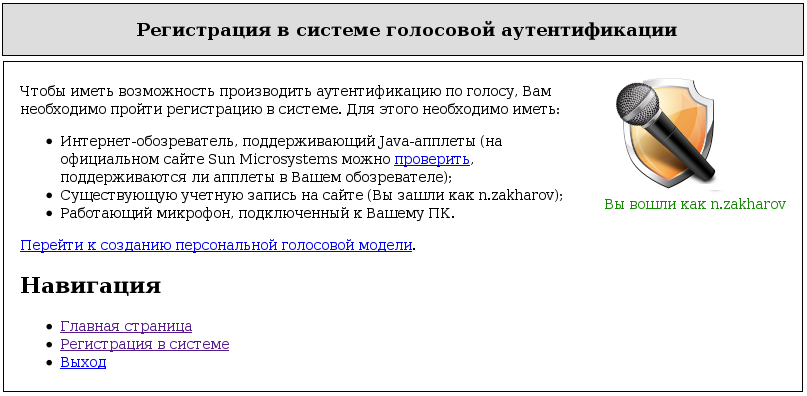
\includegraphics{static_include/enrollment_initial_authentificated.png}}
\caption{Информация о регистрации (пользователь авторизован)}
\label{fig:enrollment_initial_authentificated}
\end{figure}

\begin{figure}[hbt!]
\center{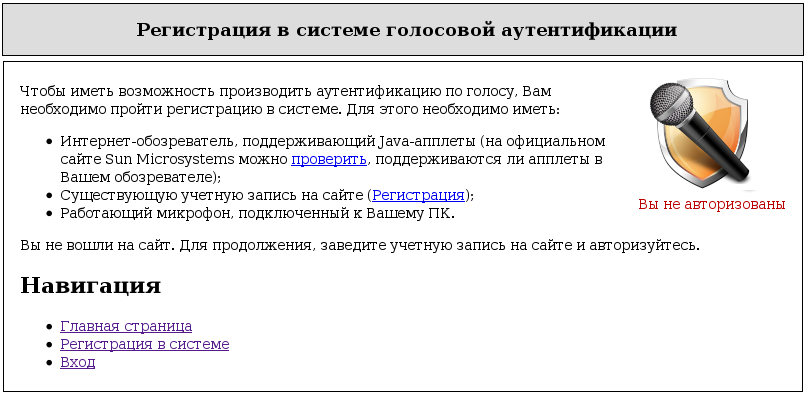
\includegraphics{static_include/enrollment_initial_anonymous.png}}
\caption{Информация о регистрации (пользователь не авторизован)}
\label{fig:enrollment_initial_anonymous}
\end{figure}

\subsubsection{Создание индивидуальной голосовой модели}
\label{sec:manual:enrollment}

В случае выбора ссылки "Перейти к созданию индивидуальной голосовой модели", производится переход к странице с формой, которая представлена на рисунке~\ref{fig:enrollment_created}. В центральной части формы нахоится краткая инструкция по записи образца ключевой фразы. В нижней части находится кнопка "Возврат", при выборе которой происходит автоматический переход на главную страницу системы голосовой аутентификации, и кнопка "Запись".


\begin{figure}[hbt!]
\center{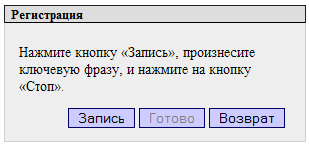
\includegraphics{static_include/enrollment_created.png}}
\caption{Регистрация: инициализация сессии записи}
\label{fig:enrollment_created}
\end{figure}

При выборе кнопки "Запись" начинается запись, и форма  автоматически переходит в состояние, изображенное на рисунке~\ref{fig:enrollment_recording}. В центральной части формы отражается состояние времени записи. В нижней части, заменяя кнопку "Запись", появляется кнопка "Стоп", при нажатии на которую происходит остановка записи.


\begin{figure}[hbt!]
\center{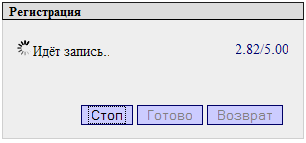
\includegraphics{static_include/enrollment_recording.png}}
\caption{Регистрация: запись голосового образца}
\label{fig:enrollment_recording}
\end{figure}

Если записанный образец слишком короткий, то при выборе кнопки "Стоп", форма переходит в состояние, представленное на рисунке~\ref{fig:enrollment_too_short_to_upload}. В центре формы находится сообщение о длительности образца и рекомендации пользователю. Из данной формы можно перейти в состояние записи голосового образца или вернуться на главную страницу системы голосовой аутентификации.


\begin{figure}[hbt!]
\center{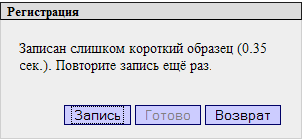
\includegraphics{static_include/enrollment_too_short_to_upload.png}}
\caption{Регистрация: недостаточно данных для отправления}
\label{fig:enrollment_too_short_to_upload}
\end{figure}

Если образец имеет достаточную длину, форма (рисунок~\ref{fig:enrollment_recording}) переходит в состояние, представленное на рисунке~\ref{fig:enrollment_uploading}. В этом состоянии происходит отпрвление записи, что отражается в  центральной части формы, также там отражено время последней записи. 


\begin{figure}[hbt!]
\center{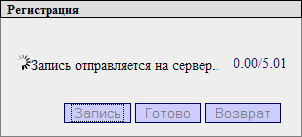
\includegraphics{static_include/enrollment_uploading.png}}
\caption{Регистрация: отправление записи}
\label{fig:enrollment_uploading}
\end{figure}


При возникновении ошибки во время отправления записи, форма переходит в состояние, представленное на рисунке~\ref{fig:enrollment_upload_error}. В центральной части формы расположено сообщение об ошибке и рекомендации пользователю. 


\begin{figure}[hbt!]
\center{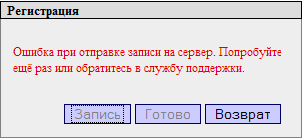
\includegraphics{static_include/enrollment_upload_error.png}}
\caption{Регистрация: ошибка при отправлении записи}
\label{fig:enrollment_upload_error}
\end{figure}



При удачном завершении отправления записи на сервер, форма (рисунок~\ref{fig:enrollment_uploading}) переходит в состояние, изображенное на рисунке~\ref{fig:enrollment_uploaded}. На форме отражается количество, общая длительность записей, и сообшение о состоянии записи. Если пользователь хочет отменить процесс регистрации, необходимо выбрать кнопку "Возврат". Если пользователь хочет продолжить создание голосовой модели, необходимо выбрать кнопку "Запись". Когда пользователь запишит достаточное количество образцов ключевой фразы, становиться активной кнопка "Готово".


\begin{figure}[hbt!]
\center{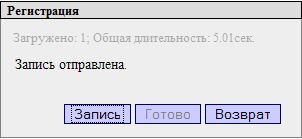
\includegraphics{static_include/enrollment_uploaded.png}}
\caption{Регистрация: запись отправлена}
\label{fig:enrollment_uploaded}
\end{figure}

При выборе кнопки "Готово" начинается процесс обучения модели, и форма переходит в состояние, представленное на рисунке~\ref{fig:enrollment_in_process}. В центральной части формы расположено сообщение о состоянии процесса обучения.

\begin{figure}[hbt!]
\center{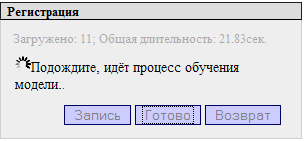
\includegraphics{static_include/enrollment_in_process.png}}
\caption{Регистрация: обучение модели}
\label{fig:enrollment_in_process}
\end{figure}

Если произошла ошибка при обучении модели, форма переходит в состояние, отраженное на рисунке~\ref{fig:enrollment_error_in_learning}. В центре формы отображается сообщение об ошибке и рекомендации пользователю. При возникновении данной ошибки, пользователь может вернуться на главную страницу системы голосовой аутентификации.

\begin{figure}[hbt!]
\center{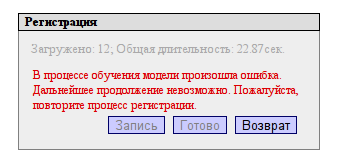
\includegraphics{static_include/enrollment_error_in_learning.png}}
\caption{Регистрация: ошибка во время обучения модели}
\label{fig:enrollment_error_in_learning}
\end{figure}

Если данных для обучения недостаточно, форма (рисунок~\ref{fig:enrollment_in_process}) переходит в состояние, показанное на рисунке~\ref{fig:enrollment_need_more_data}. В центральной части формы отображается сообщение об ошибке и рекомендации пользователю. При возникновении данной ошибки, пользователь может выбрать кнопку "Возврат" или записать дополнительные голосовые данные, выбрав кнопку "Запись".


\begin{figure}[hbt!]
\center{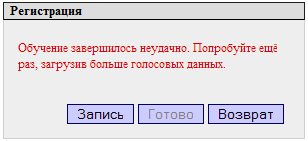
\includegraphics{static_include/enrollment_need_more_data.png}}
\caption{Регистрация: недостаточно данных для обучения модели}
\label{fig:enrollment_need_more_data}
\end{figure}

При удачном завершении обучения модели, регистрация завершается, и форма (рисунок~\ref{fig:enrollment_in_process}) переходит в состояние, показанное на рисунке~\ref{fig:enrollment_success}. Из этого состояния происходит переход на главную страницу системы голосовой аутентификации, что отражается в сообщении.   


\begin{figure}[hbt!]
\center{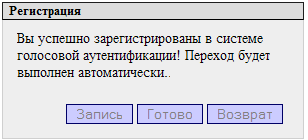
\includegraphics{static_include/enrollment_success.png}}
\caption{Регистрация: успешное завершение обучения модели}
\label{fig:enrollment_success}
\end{figure}

\subsubsection{Аутентификация по голосу}
\label{sec:manual:verification}


Если на главной странице системы голосовой аутентификации не введено имя учётной записи, то при переходе по  ссылке "Вход в систему по голосу", возникает окно с предупреждением (рисунок~\ref{fig:warning_need_login}). Если имя учётной записи введено, производится переход к странице с формой, которая представлена на рисунке~\ref{fig:verification_created}. Центральная часть формы и функция кнопки "Запись" аналогичны описанным в разделе~\ref{sec:manual:enrollment} (рисунок~\ref{fig:enrollment_created}). В нижней части формы находится кнопка "Возврат", при выборе которой, производится переход на главную страницу защищаемого интернет-ресурса.


\begin{figure}[hbt!]
\center{\includegraphics{static_include/need_login.png}}
\caption{Предупреждение о необходимости ввода имени учётной записи}
\label{fig:warning_need_login}
\end{figure}


\begin{figure}[hbt!]
\center{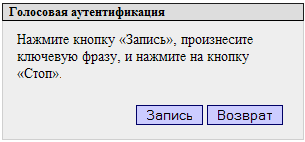
\includegraphics{static_include/verification_created.png}}
\caption{Аутентификация: инициализация сессии записи}
\label{fig:verification_created}
\end{figure}

Процесс записи ключевой фразы для аутентификации аналогичен процессу записи ключевых фраз для создания индивидуальной голосовой модели. Различие заключается в том, что запись производится один раз, после чего начинается процесс аутентификации (рисунок~\ref{fig:verification_in_process}). 


\begin{figure}[hbt!]
\center{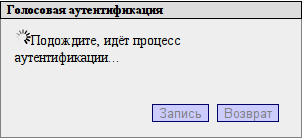
\includegraphics{static_include/verification_in_process.png}}
\caption{Аутентификация: процесс аутентификации}
\label{fig:verification_in_process}
\end{figure}

Если во время аутентификации произошла ошибка , форма переходит в состояние, отраженное на рисунке~\ref{fig:verification_error}. В центре формы отображается сообщение об ошибке и рекомендации пользователю. При возникновении данной ошибки, пользователь может повторить попытку аутентификации, выбрав кнопку "Повтор", или перейти на главную страницу интернет-ресурса, выбрав кнопку "Возврат". 


\begin{figure}[hbt!]
\center{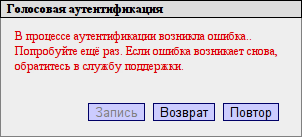
\includegraphics{static_include/verification_error.png}}
\caption{Аутентификация: ошибка во вермя аутентификации}
\label{fig:verification_error}
\end{figure}

Если процесс аутентификации завершился отказом в доступе, форма (рисунок~\ref{fig:verification_in_process}) переходит в состояние, показанное на рисунке~\ref{fig:verification_access_denied}. В центре формы отображается сообщение о состоянии аутентификации и рекомендации пользователю. В нижней части формы находятся кнопки "Возврат" и "Повтор".


\begin{figure}[hbt!]
\center{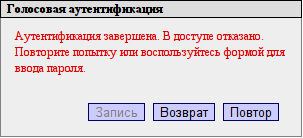
\includegraphics{static_include/verification_access_denied.png}}
\caption{Аутентификация: в доступе отказано}
\label{fig:verification_access_denied}
\end{figure}

Если аутентификация завершается успешно для пользователя (доступ разрешён), происходит автоматический переход на запрошенную страницу, или на страницу, заданную по-умолчанию, администратором интернет-ресурса.  

\subsubsection{Интерфейс администратора}

На главной странице интерфейса администратора представлен список разделов, отвечающих за управление соответствующими объектами системы (рисунок~\ref{fig:admin_main}). Все перечисленные объекты подробно описаны в разделе~\ref{} 

\begin{figure}[hbt!]
\center{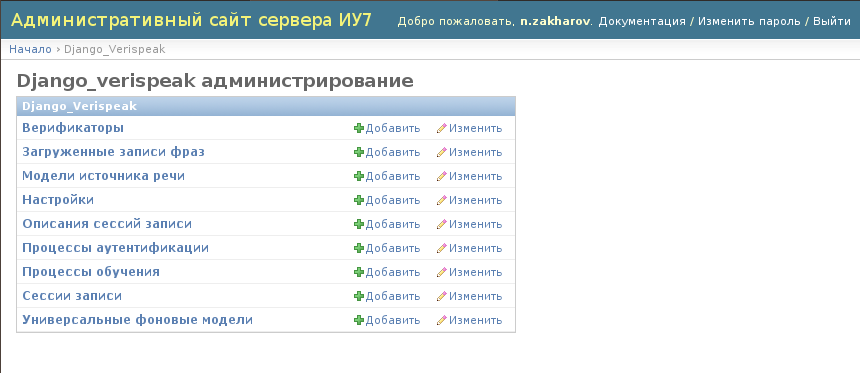
\includegraphics[width=0.8\textwidth]{include/admin_main.png}}
\caption{Главное окно интерфейса администратора}
\label{fig:admin_main}
\end{figure}












